\subsection{Training}
\label{sec:neural-networks-training}
Thus far optimal weights and biases were assumed in all examples.
But in practical terms they need to be found first.
This starts by generating and preparing a dataset from which the network can find correlations.
Based on this, the weights and biases are adapted step wise.
Each of these steps is covered in the following sections.

\subsubsection{Dataset Generation}
\label{sec:dataset-generation}
The whole training process is based on the dataset from which the network learns the correlations of input and label.
Usually, a dataset consists of input-label pairs, where the input is the data that is fed into the network and the label is the ground-truth.
In the case of a classification task, the label represents the category.
However, there is no general rule for the amount of data.
It can be said, that more data is better for generalization, but too many samples can lead to overfit the network to the shown data.
The latter means, that the network is trained to long or to intensive on the shown data.
The consequence is, that it adjusts its weights and biases to classify this data perfectly, but cannot reliably classify general, unknown data of same objects anymore, because they slightly differ.
Basically, the amount of data depends on the objective of the network.
For classifying whether an image is black or white, only a few training samples would be needed.
Is the objective classifying objects within images, it depends on the number of possible objects and their complexity.
If the objects are simple geometric shapes, then not as many samples are needed as if the objects are common objects like type of animals or cars.
For the latter the number of samples would probably be approximately 1000 examples per class.
Luckily, there are several datasets available, that are already sorted and labeled, like the MNIST handwritten digits or the ImageNet dataset.
Available datasets are not limited to images, but can contain CAD models like the ModelNet dataset which is used for this network architecture.

Samples of a dataset are split into a training and testing set, and sometimes a validation set\cite{James2014}.
The first contains data, the network trains on.
From this data correlations of input and label are found.
After arbitrary training steps where parameter changes happened, the performance of the network is tested on the validation set.
This is data, the network is not trained on.
The objective is to check if overfitting occurs.
If the accuracy of the training set increases, the accuracy of the validation set has to increase as well.
This shows that the network still learns and gets better.
If the accuracy of the training set increases, but the accuracy of the validation set stays the same or decreases, it is an indicator for overfitting.
The testing set is data the network is not trained on as well.
It serves as a final performance check of the network to confirm its general accuracy.
If no validation set is available, the testing set can be used.
How the dataset is split depends again on the number and complexity of samples and the objective.
However, a equal distribution of samples in each set should be minded.
Otherwise the performance will not be satisfying.
This means, if the network trains mostly on sweatshirts a test set with mostly pants would not yield an acceptable accuracy, because the network does not know these particular features.

For processing the dataset, a one-hot encoding\cite{Harris2012} of the labels is recommended.
Usually, the labels are categorical data.
This means, they contain label or string values, respectively, instead of numeric values, that the networks needs.
For example, there is a fashion variable with the values "boot", "sweatshirt" and "pants".
The network would not know how to interpret these.
Thus, these values need to be converted to numeric values.
Furthermore, if these label values are outputs of the network, it should be easily possible to convert them back from numeric values.
Hence, they are converted to integers that represent a category.
Referring to the example, this results in the numeric values 0, 1 and 2 for the labels "boot", "sweatshirt" and "pants", respectively.
But numeric values have a natural ordered relationship between each other, that neural networks could exploit.
The index of "pants" is higher than the one of "boot", but neither of these categories is better or worse than the other.
Therefore, the indices are one-hot encoded as well.
This means removing the integer representation and inserting binary variables for simulating existing features.
Applying this to the example results in the feature label vector $\vec{f}_1 = (0, 1, 0)^T$ for the "sweatshirt" label.
This vector has a length of the number of different categories available, where every element is 0 except the one of the corresponding category which is 1.
\tabref{tab:one-hot-encoding} summarizes this approach.
\begin{table}[]
	\caption[One-Hot Encoding of Categorical Data]{One-hot encoding of categorical data. First, categorical label values are transformed to numeric values representing a category index. Then, this is replaced with binary variables to represent features, that removes the natural relationship of numeric values to each other. This vector has a length of the number of different categories, where every element is 0 except for the corresponding category which is 1.}
	\label{tab:one-hot-encoding}
	\centering
	\begin{tabular}{l|l|l}
		Categorical   & Integer & One-Hot                   \\ \hline
		"Boot"       & 0       & $\vec{f}_0 = (1, 0, 0)^T$ \\
		"Sweatshirt" & 1       & $\vec{f}_1 = (0,1, 0)^T$  \\
		"Pants"      & 2       & $\vec{f}_2 = (0, 0, 1)^T$
	\end{tabular}
\end{table}
\subsubsection{Stochastic Gradient Descent}
\label{sec:training-stochastic-gradient}
Let's recall the information, that are needed for the actual training step, i.e. the finding of optimal weights and biases.
Everything starts with a dataset $\mathbb{D}$ containing $m$ pairs of inputs and corresponding labels.
Performing a one-hot encoding on the labels yields by assuming in general flattened input matrices
\begin{equation}
	\label{eq:dataset-one-hot}
	\mathbb{D} =
	\begin{pmatrix}
		\vec{X} & \vec{Y}
	\end{pmatrix}
\end{equation}
where $\vec{X} \in \mathbb{R}^{n_x \times m}$ and $\vec{Y} \in \mathbb{R}^{n_y \times m}$ are representing each input and label as vectors, respectively.
Hereby, $n_x$ represents the size of each input and $n_y$ the number of categories.
Furthermore, there is a neural network with $L$ layers each containing an arbitrarily number of perceptrons.
Expressing the activation of every node with \thmref{eq:perceptron-sum} would get very confusing for a whole network.
Hence, a matrix notation is the way to go in the long run.
First, for every $j$-th node in the $l$-th layer its weights are summarized in a vector
\begin{equation}
	\label{eq:weights-vector}
	\vec{w}^{[l]}_j =
	\begin{pmatrix}
		w^{[l]}_{j,0} & w^{[l]}_{j,1} & \cdots & w^{[l]}_{j,n^{[l-1]}_h}
	\end{pmatrix}^T
\end{equation}
containing single weights, where the superscript in square brackets denotes the layer and the subscript denotes the edge of (target neuron, preceding neuron).
The number of hidden neurons in the $l$-th layer is represented by $n^{[l]}_h$.
These conventions are maintained for all parameters for the rest of this thesis.
The bias is just a scalar denoted as $b^{[l]}_j$. 
Now, every weight vector and bias can be combined to a matrix and vector, respectively, for each layer.
This yields
\begin{subequations}
\label{eq:parameters}
	\begin{align}
		\vec{W}^{[l]} &=
		\begin{pmatrix}
			\vec{w}^{[l]}_0 & \vec{w}^{[l]}_1 & \cdots & \vec{w}^{[l]}_{n^{[l]}_h}
		\end{pmatrix}^T
		\label{eq:weights}
		\\
		\vec{b}^{[l]} &=
			\begin{pmatrix}
				b^{[l]}_0 & b^{[l]}_1 & \cdots & b^{[l]}_{n^{[l]}_h}
			\end{pmatrix}^T
		\label{eq:biases}
	\end{align}
\end{subequations}
where $\vec{W}^{[l]} \in \mathbb{R}^{n^{[l]}_h \times n^{[l-1]}_h}$ and $\vec{b}^{[l]} \in \mathbb{R}^{n^{[l]}_h}$.

Using these matrices and vectors data can easily be forwarded through the network by building up on \thmref{eq:perceptron-activation}.
The weighted sum of all neurons of the $l$-th layer is computed as
\begin{equation}
	\label{eq:weighted-sum}
	\vec{z}^{[l]} = \vec{W}^{[l]} \vec{a}^{[l-1]} + \vec{b}^{[l]}
\end{equation}
with the activations vector $\vec{a}$.
Putting this in an activation function yields
\begin{equation}
	\label{eq:activations}
	\vec{a}^{[l]} = \phi\left(\vec{z}^{[l]}\right)
\end{equation}
for the $l$-th layers activations.
Performing this for every layer results in 
\begin{equation}
	\label{eq:feedforward}
	\hat{\vec{y}} = f(\vec{x}^{(i)})
\end{equation}
as the networks prediction, where $\vec{x^}{(i)} \in \mathbb{R}^{n_y}$ is the $i$-th data sample.
This superscript in round brackets is part of the used convention.

Let's assume that the result is already fed into a sigmoid function and therefore only contains values between 0 and 1.
This prediction needs to be compared with the ground-truth label $\vec{y}^{(i)}$ for checking how good the network performs and, hence, how well the parameters fit.
An example of how these vectors can look like is shown in \tabref{tab:prediction}.
\begin{table}[]
	\centering
	\caption[Example Comparison of One-Hot Encoded Ground Truth Label and Prediction]{Example comparison of an one-hot encoded ground truth label and a prediction. However, the actual ground truth feature has the second smallest probability in the prediction. Therefore, the parameters need to be adjusted.}
	\label{tab:prediction}
	\begin{tabular}{ll}
		Ground-Truth & $\vec{y} = \begin{pmatrix} 0 & 1 & 0 & 0 & 0 \end{pmatrix}^T$                     \\
		Prediction   & $\hat{\vec{y}} = \begin{pmatrix} 0.54 & 0.28 & 0.2 & 0.63 & 0.96 \end{pmatrix}^T$
	\end{tabular}
\end{table}
It can be clearly seen, that the prediction is completely wrong.
The actual ground truth feature has the second smallest probability in the prediction.
In theory, an identical representation would be desirable.
However, in practical terms a slight deviation is normal.
Because finding optimal parameters is a optimization problem, a metric for the performance of the networks is served by a loss function that maps these parameters to a cost.
The most common loss function for mutually exclusive classes is the cross entropy loss function.
It is defined as
\begin{equation}
	-(y \log(p) + (1-y) \log(1-p))
\end{equation}
for two classes and as
\begin{equation}
	\label{eq:cross-entropy}
	H(\vec{y}, \vec{p}) = - \sum_{i}^{M} y_i \log (p_i)
\end{equation}
for multiclass classification, where $M$ is the number of classes, $i$ the moving index, $\vec{y}$ the ground truth vector and $\vec{p}$ the predicted probabilities.
Adapting the previous notation to this yields
\begin{align}
	\vec{y} &= \vec{Y}^{(i)} \\
	\vec{p} &= \hat{\vec{y}} \\
	M &= n_y
\end{align}
as analogies.
%TODO insert figure of cross entropy graph
%TODO because of one hot only one parameter is relevant
\subsubsection{Adam: Adaptive Moment Estimation}
\label{sec:training-adam}
Learning rate schedules have the problems of defining their parameters in advance and applying the same learning rate to every weight and bias.
Hence, the RMSProp (Root Mean Square Propagation) optimizer was developed\cite{Tieleman2012}.
Its objective is illustrated in \figref{fig:rmsprop}.
The ellipses represent contour lines.
The orange line visualizes the process of gradient descent.
Using it can result in parameters oscillating in one direction while making progress in another one moving to the minimum.
The objective of RMSProp, represented by the blue line, tries to dampen the oscillations by slowing down learning of the responsible parameter and fasten up the other one.
Hence, it can use a larger learning rate and reaches the minimum more quickly.
\begin{figure}
	\centering
	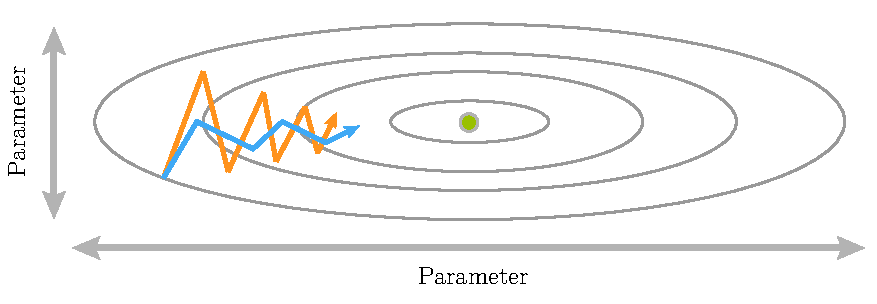
\includegraphics[]{images/rmsprop.pdf}
	\caption[Process of gradient descent and RMSProp]{Process of gradient descent and RMSProp using contour lines. The orange line illustrates the process of gradient descent. It oscillates and moves slowly to the minimum. The blue line shows the process of the RMSProp algorithm. While one parameter changes slower the other one changes faster. Hence, it dampens oscillations and moves faster to the minimum.}
	\label{fig:rmsprop}
\end{figure}
RMSProp adapts a learning rate to each of the parameters.
Furthermore, it divides the learning rate for a parameter by a weighted running average of the magnitudes of its previous gradients.
The weighted running average is calculated by
\begin{subequations}
	\label{eq:adam-second-momentum}
	\begin{align}
		v(w^{[l]}_{jk}, \tau) &= \beta_2 v(w^{[l]}_{jk}, \tau - 1) + (1-\beta_2) (\nabla \vec{J}(w^{[l]}_{jk}))^2 \\
		v(b^{[l]}_{j}, \tau) &= \beta_2 v(b^{[l]}_{j}, \tau - 1) + (1-\beta_2) (\nabla \vec{J}(b^{[l]}_{j}))^2
	\end{align}
\end{subequations}
where hyperparameter $\beta_2$ is the forgetting factor.
As a value, its author suggests $\beta_2 = 0.9$.
The subscript $2$ is for later purposes and could be omitted for now.
The squaring operation is done element-wise.
So this expression adds kind of inertia to the update procedure dampening oscillations and building up speed on flat surfaces.
Finally, the parameters are updated by
\begin{subequations}
	\begin{align}
		w^{[l]}_{jk} &:= w^{[l]}_{jk} - \frac{\gamma}{\sqrt{v(w^{[l]}_{jk}, \tau)}} \nabla \vec{J}(w^{[l]}_{jk}) \\
		b^{[l]}_{j} &:= b^{[l]}_{j} - \frac{\gamma}{\sqrt{v(b^{[l]}_{j}, \tau)}} \nabla \vec{J}(b^{[l]}_{j})
	\end{align}
\end{subequations}
using the weighted moving average just calculated.
Let's say the horizontal parameter is $w_1$ and the vertical one $w_2$ referring to \figref{fig:rmsprop}.
Due to the oscillations, the gradient $\nabla \vec{J}(w_2)$ is much larger than $\nabla \vec{J}(w_1)$.
Hence, $v_2$ is larger than $v_1$ resulting in a smaller update for $w_2$ and a larger one for $w_1$.
This yields a more direct moving to the minimum.
However, this approach does not make it easier to configure the learning rate as the step size is independent of it.
Though, it improves the speed of the optimization process because a better set of weights is discovered in fewer training steps than with pure gradient descent.
The Adam (Adaptive Moment Estimation) optimization is an update to the RMSProp algorithm by adding a momentum
\begin{subequations}
	\label{eq:adam-first-momentum}
	\begin{align}
		m(w^{[l]}_{jk},\tau) &= \beta_1 m(\tau -1) + (1- \beta_1) \frac{\partial J}{\partial w^{[l]}_{jk}} \\
		m(b^{[l]}_{j},\tau) &= \beta_1 m(\tau -1) + (1- \beta_1) \frac{\partial J}{\partial b^{[l]}_{j}}
	\end{align}
\end{subequations}
for each parameter using a weighted average of the latest gradients\cite{DBLP:journals/corr/KingmaB14} where $\beta_1$ is the forgetting factor.
This momentum can be imagined as a ball in a bowl-shaped cost function rolling downwards and building up speed depending on the gradients.
The hyperparameter $\beta_1$ represents friction.
This approach can be summarized by using running averages of both the gradients and the second moments of the gradients.
Due to the initialization $\vec{v} = \vec{0}$ and $\vec{m} = \vec{0}$ these values are biased towards zero, especially during the first few iterations.
A correction is desirable because the first and second moments are only estimations.
In general, an estimation should equal the parameter that is tried to be estimated.
Hence, the property
\begin{subequations}
	\begin{align}
		E[m] &= E[g]\\
		E[v] &= E[g^2]
	\end{align}
\end{subequations}
needs to be fulfilled, where $E[\cdot]$ represents the expectation of a variable.
These properties only hold true, if unbiased estimators are used.
Hence, the corrected values are expressed by
\begin{subequations}
	\label{eq:adam-corrected}
	\begin{align}
	\hat{m}(w^{[l]}_{jk}, \tau) &= \frac{m(w^{[l]}_{jk},\tau)}{1-\beta_1^\tau} \\
	\hat{m}(b^{[l]}_{j}, \tau) &= \frac{m(b^{[l]}_{j},\tau)}{1-\beta_1^\tau} \\
	\hat{v}(w^{[l]}_{jk}, \tau) &= \frac{v(w^{[l]}_{jk}, \tau)}{1-\beta_2^\tau} \\
	\hat{v}(b^{[l]}_{j}, \tau) &= \frac{v(b^{[l]}_{j}, \tau)}{1-\beta_2^\tau}
	\end{align}
\end{subequations}
using the expression from before.
Finally,
\begin{subequations}
	\label{eq:adam-update}
	\begin{align}
		w^{[l]}_{jk} := w^{[l]}_{jk}-\gamma \frac{\hat{m}(w^{[l]}_{jk})}{\sqrt{\hat{v}(w^{[l]}_{jk})} + \epsilon} \\
		b^{[l]}_{j} := b^{[l]}_{j}-\gamma \frac{\hat{m}(b^{[l]}_{j})}{\sqrt{\hat{v}(b^{[l]}_{j})} + \epsilon}
	\end{align}
\end{subequations}
updates the parameters, where $\epsilon$ is a small constant for preventing a division by zero.
As for other optimization algorithms the learning rate $\gamma$ needs to be tuned.
The remaining hyperparameters are recommended by \textit{Kingma et al.} to be $\beta_1 = 0.9$, $\beta_2 = 0.999$ and $\epsilon = 10^{-8}$.
However, the latter has no big impact on the optimization.

Expressing the activation of every node with \thmref{eq:perceptron-sum} would get very complex with only a few nodes.
Hence, a matrix notation is the way to go in the long run.
First, for every layer a vector is build